%-------------------------------------------------------------------------
% PACKAGES AND OTHER DOCUMENT CONFIGURATIONS
%-------------------------------------------------------------------------

\documentclass[11pt]{article}
%----------------------------------------------------------------------------------------------
%   PACKAGES AND CONFIGURATIONS 
%----------------------------------------------------------------------------------------------

\usepackage{lastpage}
\usepackage{hyperref}
\usepackage{graphicx}
\usepackage{pgfplots}
\pgfplotsset{compat=1.17}
\usepackage{xcolor}
\usepackage{amsmath}
\usepackage{bussproofs}
\usepackage{amssymb}
\usepackage{amsfonts}
\usepackage{graphicx}
\usepackage{booktabs}
\usepackage{listing}
\usepackage{etoolbox}
\usepackage{latexsym}
\usepackage{listings}
\usepackage[utf8]{inputenc}
\usepackage{caption}
\graphicspath{{./img}}

\DeclareCaptionFont{white}{\color{white}}
\DeclareCaptionFormat{listing}{%
  \parbox{\textwidth}{\colorbox{gray}{\parbox{\textwidth}{#1#2#3}}\vskip-4pt}}
\captionsetup[lstlisting]{format=listing,labelfont=white,textfont=white}
\lstset{frame=lrb,xleftmargin=\fboxsep,xrightmargin=-\fboxsep}

%-----------------------------------------------------------------------------------------------
%   MARGINS
%-----------------------------------------------------------------------------------------------

\usepackage{geometry}
\geometry{
    paper=a4paper,
    top=3cm,
    bottom=3cm,
    left=2.5cm,
    right=2.5cm,
    headheight=14pt,
    footskip=1.4cm,
    headsep=1.2cm,
}

%-----------------------------------------------------------------------------------------------
%   FONT
%-----------------------------------------------------------------------------------------------

\usepackage[utf8]{inputenc}
\usepackage[T1]{fontenc}

\usepackage[sfdefault,light]{roboto}

%-----------------------------------------------------------------------------------------------
%   HEADER AND FOOTER   
%-----------------------------------------------------------------------------------------------

\usepackage{fancyhdr}
\pagestyle{fancy}

\lhead{\small\classHomework\ifdef{\className}{\ (\className):}{}\ \homeworkTitle}
\chead{}
\rhead{\small\ifdef{\authorName}{\authorName}{\ifdef{dueDate}{Due\ \dueDate}{}}}

\lfoot{}
\cfoot{\small Page\ \thepage\ of\ \pageref{LastPage}}
\rfoot{
\includegraphics[scale=0.06]{logo-unige.png}}

\renewcommand\headrulewidth{0.5pt}

%-------------------------------------------------------------------------------------------------
%   TITLE PAGE
%-------------------------------------------------------------------------------------------------

\author{\textbf{\authorName}}
\date{}

\title{
    \thispagestyle{empty}
    \vspace{0.2\textheight}
    \textbf{\classHomework:\ \homeworkTitle}\\[-4pt]
    \ifdef{\classHomework}{{\small Due\ on\ \dueDate}\\}{}
    \ifdef{\className}{{\large \textit{\className}}}{}
    \vspace{0.32\textheight}

    
\includegraphics[scale=0.2]{logo-unige.png}
}
 % Ensure this file contains all necessary package inclusions and settings

%-------------------------------------------------------------------------
% HOMEWORK INFORMATION
%-------------------------------------------------------------------------

\newcommand{\classHomework}{13X007}
\newcommand{\homeworkTitle}{Assignment\ \#3}
\newcommand{\authorName}{CHRISTOFOROU Anthony}
\newcommand{\className}{Parallelism}
\newcommand{\dueDate}{08.11.2023}

%-------------------------------------------------------------------------

\begin{document}
    
    \maketitle
    \thispagestyle{empty}
    \newpage

    \begin{abstract}
        This report investigates the parallelization of a 2D heat equation solver using the Message Passing Interface (MPI). The Finite Difference Method with the Forward-Time Centered-Space (FTCS) scheme was applied across different domain sizes. Performance was analyzed by timing executions across a range of processor counts. The results demonstrate the power of parallel computing to significantly reduce computation time, particularly for large domain sizes, while also highlighting the trade-offs and challenges associated with parallelization, such as communication overhead and load balancing. The study provides insights into optimizing parallel computation strategies, contributing to the broader field of computational science.
    \end{abstract}

    \tableofcontents
    
    \newpage
    
    \section{Introduction}
        The 2D heat equation is a fundamental partial differential equation that describes heat conduction. It represents how heat diffuses through a given area over time. This report details the application of parallel computing techniques, specifically MPI, to solve the equation more efficiently. It discusses the methods used, the results obtained, and the insights gained from the process, highlighting the importance of parallelism in computational science.

        \subsection{Background}
        The heat equation is central to thermal physics and engineering, providing insight into the thermal behavior of materials and systems. Its solutions are crucial for designing heat management systems in various engineering disciplines, from electronics to aerospace.

        \subsection{Significance of Parallel Computing}
        Traditional serial computation methods become impractical as the complexity and size of the domain increase. Parallel computing addresses this by splitting the task among multiple processors, leading to substantial reductions in computation time and enabling the solution of larger and more complex problems.

    \section{Methodology}
        This section outlines the computational approach used to solve the 2D heat equation, detailing the numerical method employed and the parallelization technique.

        \subsection{Finite Difference Method}
        The Finite Difference Method (FDM) approximates the continuous differential equations of the heat equation with a discretized grid. The grid spacing and time step size were chosen according to the stability criteria of the FTCS scheme. Boundary conditions were set to maintain a constant temperature at the edges of the domain, representing a typical physical scenario.

        \subsection{Parallelization Strategy}
        The domain was decomposed into subdomains assigned to different processors. The MPI framework facilitated communication between processors, allowing for efficient data exchange necessary for boundary condition calculations and iterative updates.

        \subsection{Computational Setup}
        The computations were performed on a computer equipped with a Ryzen 9 3900X CPU 12 Core Processor.

    \section{Results}
        The following subsections present the empirical data gathered from the simulations, highlighting the performance improvements and providing a detailed analysis of the results.

        \subsection{Execution Time Measurements}
        Execution times were recorded for domain sizes 64x64, 128x128, and 256x256 with varying processor counts. A general reduction in computation time was observed with the increase in processor count.

        \subsection{Graphical Representation}
        The data were plotted using line graphs, which clearly show the trend of decreasing execution time with an increasing number of processors. These graphs provide an immediate visual representation of the performance gains achieved through parallelization. This was made with a ver large number of iteration ($10^5$) as less than this would have been too fast therefore the communication between the processors would have been too important, because there would have been too many communications for a small amount of computation.

    \begin{figure}[ht]
        \centering
        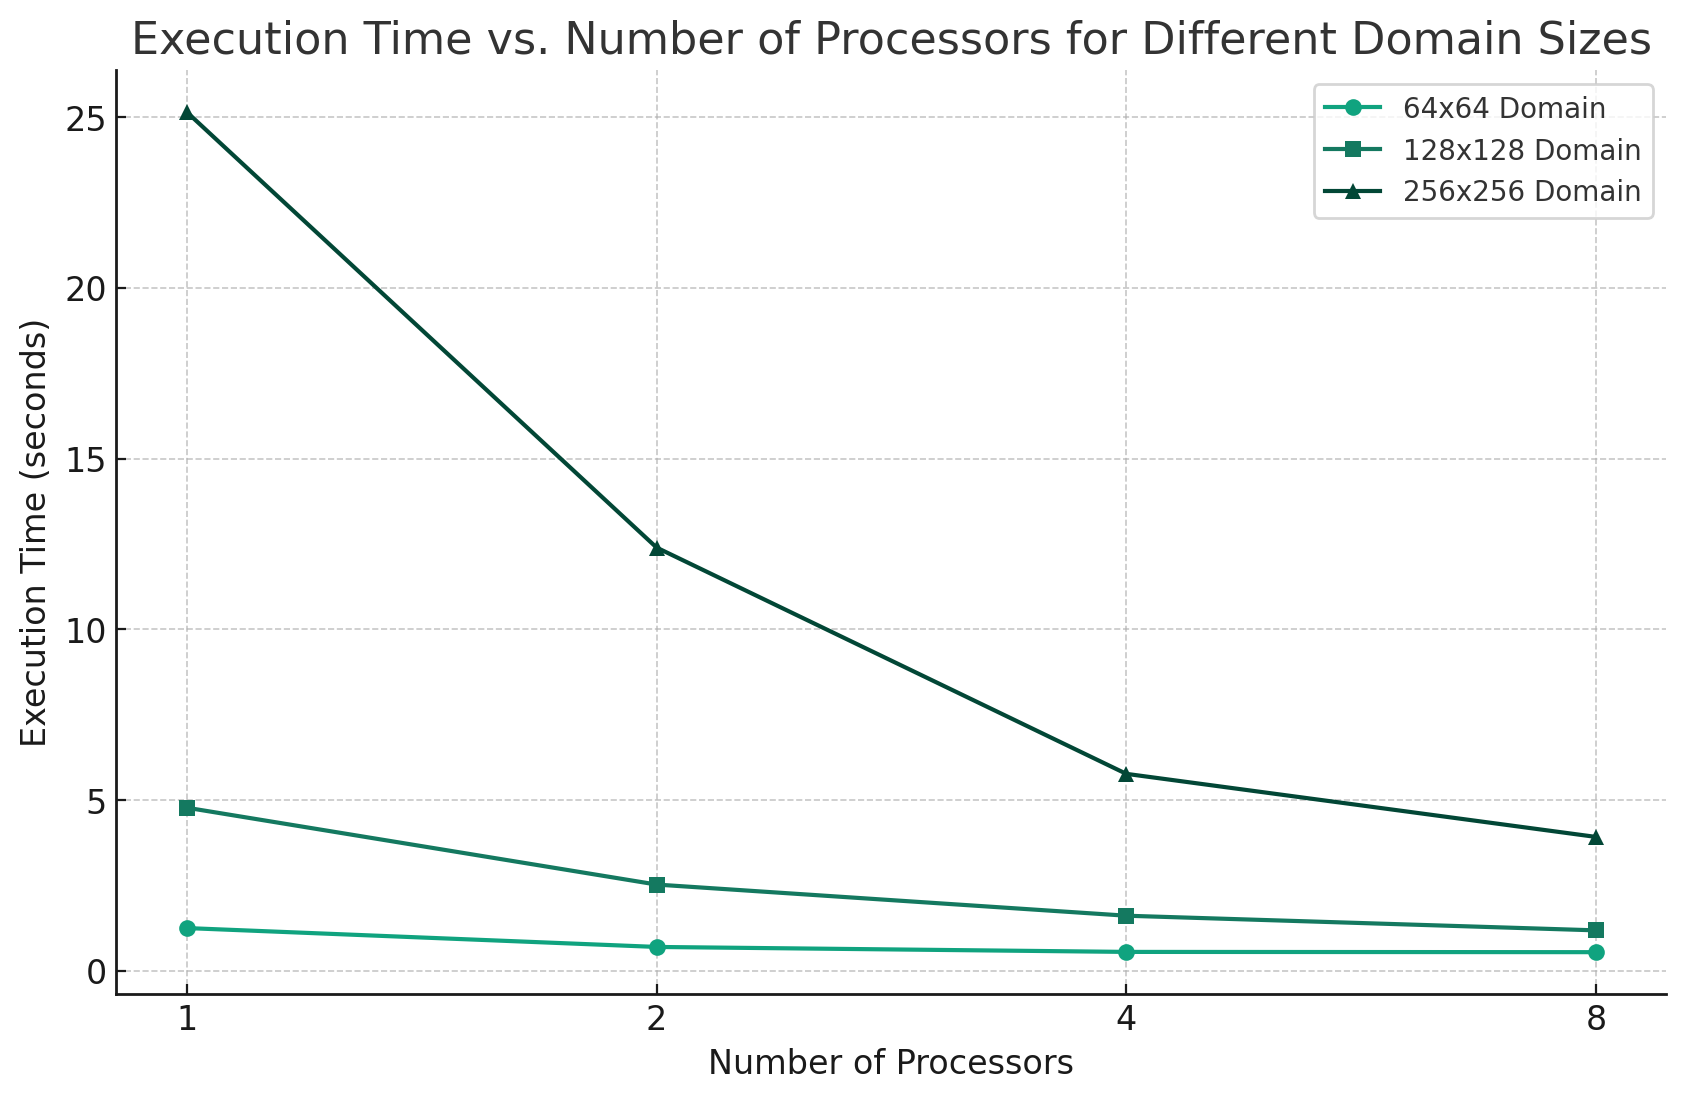
\includegraphics[width=0.8\textwidth]{img/performance.png}
        \caption{Execution Time vs. Number of Processors for Different Domain Sizes}\label{fig:execution_time}
    \end{figure}

        \subsection{Analysis of Results}
        The results indicate a trend consistent with Amdahl's Law; the speedup due to parallelization is substantial but tends to level off as the number of processors increases. This is particularly evident in the case of smaller domain sizes, where the communication overhead can offset the computational speedup.

        For example, the solver's execution time for a 64x64 domain decreased from 1.25073 seconds with one processor to 0.545042 seconds with eight processors. Similarly, for a 128x128 domain, the time reduced from 4.77483 seconds to 1.18351 seconds, and for a 128x128 domain, from 25.1451 seconds to 3.91991 seconds with the same increase in processors.

        We'll talk more about the implications of these results in the discussion section.

        \subsection{Case Study: 256x256 Grid}
        A detailed case study of the 256x256 grid provides a clear example of the solver's functionality.

        \subsubsection{Initial Heat Distribution}
    The initial grid represents the temperature distribution at the beginning of the simulation, where boundary conditions are set to 1 (representing a fixed temperature) and the interior points are initialized to 0.

    \begin{figure}[ht]
        \centering
        
\includegraphics[width=0.4\textwidth]{img/initial_grid.png}
        \caption{Initial temperature distribution on an 256x256 grid.}
        \label{fig:initial_grid}
    \end{figure}

    \subsubsection{Evolution of Heat Distribution}
    Here you'll be able to see the evolution with the number of iteration of the heat dispertion. The heat has diffused from the boundaries into the interior according to the 2D heat equation.

    \begin{figure}[ht]
        \centering
        
\includegraphics[width=0.20\textwidth]{img/T_0015.png}
        
\includegraphics[width=0.20\textwidth]{img/T_0150.png}
        
\includegraphics[width=0.20\textwidth]{img/T_0250.png}
        
\includegraphics[width=0.20\textwidth]{img/T_0500.png}
        \\[\smallskipamount]
        
\includegraphics[width=0.20\textwidth]{img/T_1000.png}
        
\includegraphics[width=0.20\textwidth]{img/T_5000.png}
        
\includegraphics[width=0.20\textwidth]{img/T_10000.png}
        
\includegraphics[width=0.20\textwidth]{img/T_15000.png}
        \caption{Temperature evolution on an 256x256 grid.}
        \label{fig:final_grid}
    \end{figure}

    \section{Discussion}
    The discussion assesses the results' implications, evaluating the benefits of parallelization and its constraints. The insights gained from this study illustrate the balance between computational speedup and parallel overhead, shaping the strategies for future parallel computing applications.

    \subsection{Performance Gains}
    The performance analysis revealed a marked improvement in computation times when using parallel processing. For instance, the solver's execution time for a 256x256 domain showed a reduction from 25.1451 seconds with a single processor to just 3.91991 seconds with eight processors, a speedup of approximately 6.42 times. This improvement emphasizes the critical advantage of parallel computing in handling large-scale problems, where the computational workload is significantly heavy. The ability to distribute this workload across multiple processors enables the handling of complex simulations that would be otherwise unfeasible in a reasonable timeframe with serial computing.

    \subsection{Challenges in Parallelization}
    However, parallelization introduces its own set of challenges, most notably load balancing and communication overhead. Load balancing refers to the equitable distribution of workload across all processors, preventing scenarios where some processors are idle while others are overloaded. In our simulations, ensuring a uniform distribution of the computational grid to processors was imperative for achieving optimal performance.

    Communication overhead became increasingly pronounced with the addition of more processors. This is because each processor must exchange boundary information with its neighbors at each iteration, which can become a bottleneck, especially for small domain sizes where the ratio of computation to communication is low. For example, when operating on a 64x64 grid, increasing the number of processors from one to eight only halved the execution time, indicating significant communication costs.

    To mitigate these challenges, we adopted strategies such as refining the granularity of domain decomposition and employing non-blocking communication to overlap computation with data exchange, thus reducing idle time.

    \subsection{Implications for Scalability}
    The scalability of our parallel solution was not linear and highlighted the nuanced nature of Amdahl's Law in practice. The law posits that the speedup of a parallel program is limited by the time needed for the sequential fraction of the task. In our context, despite the high parallelizability of the heat distribution problem, the speedup plateaued with an increasing number of processors, indicating the presence of a non-negligible sequential component in our algorithm.

    The efficiency of the MPI implementation also played a significant role in scalability. The use of advanced MPI features, such as derived data types and collective communication, proved beneficial for reducing the complexity and duration of inter-process communication.

    The computing system's architecture, specifically the interconnects between processors, determined the performance ceiling for our parallel application. A high-performance computing cluster with low-latency networking would likely exhibit different scalability characteristics compared to our Ryzen-based setup, potentially allowing for better performance with a higher number of processors.

    Overall, the trade-offs highlighted in this study between computational speedup and parallel overhead underscore the importance of a balanced approach to parallelization, one that considers the specific characteristics of the problem, the efficiency of the parallel computing framework, and the underlying hardware architecture.

    \section{Compilation and Execution}
        \subsection{Build and Compilation}
        The project uses a Makefile for compilation to simplify the build process. To compile the parallelized heat equation solver, navigate to the project directory and run the following command:
        
        \begin{verbatim}
        make
        \end{verbatim}

        This produces an executable named \texttt{heat} in the build directory.

        \subsection{Running the Solver}
        The solver can be executed using MPI with the following command pattern:
        
        \begin{verbatim}
mpirun -np [number_of_processors] ./build/heat [domain_size] [number_of_iterations]
        \end{verbatim}

    For example, to run the solver on a 128x128 domain using 4 processors, the command would be:
        
        \begin{verbatim}
        mpirun -np 4 ./build/heat 128 1500
        \end{verbatim}

        The terminal output for this command would resemble:
        
        \begin{verbatim}
        Simulation took 1.61275 seconds.
        \end{verbatim}

        The results will be output to a bmp image named \texttt{T\_[number\_of\_iterations].bmp}, containing the final temperature distributions.

    \section{Conclusion}
        The report concludes with an overview of the findings, emphasizing the significant performance gains achieved through parallelization. The importance of optimizing both the computational aspects and the communication strategies is highlighted as key to further performance improvements.

\end{document}
